\documentclass{amsart}
\usepackage{graphicx}

\begin{document}
\author{ Catherine Zuo, Kimberly Toy,and Will Oursler}
\title{Design Notes}
\date{\today}
\maketitle

This document contains rough design guidelines. These guidelines should be carefully fleshed out and discussed, both before coding, and during coding as problems become apparent.

\section{ Dependency Graph }

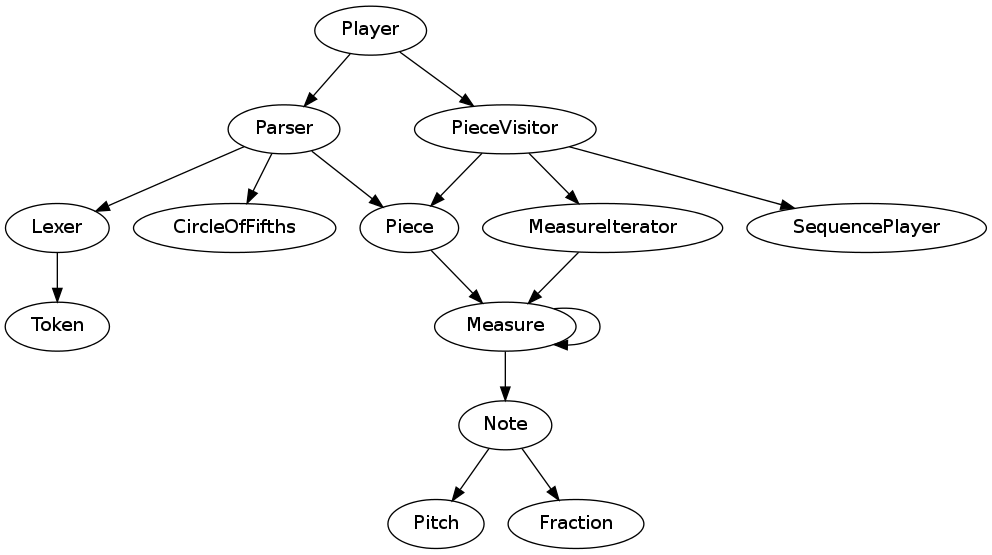
\includegraphics[width=\linewidth]{classes.png}

\section{ The Fraction class }

Because note lengths and start times are all rational numbers, and because the exact ratios of these numbers with respect to others is important, a Fraction method is useful.

The Fraction class has a Numerator and Denominator, guaranteed to be in lowest terms. It supports addition and multiplication ( possibly division and subtraction if w have time ). It will make heavy use of GCD and LCM methods, which we be from %TODO...

\section{ The Piece class }

This class is primarily concerned with the piece metadata, such as BPM, time, etc. It also contains a reference to the first Measure of the piece.  It is a mutable class and has methods to set the piece's voices.  

\section{ The Measure class and Repeats }

Each measure is a container of Note instances, each Note being associated with a start time ( represented by a Fraction ) relative the beginning of the measure. In this manner, the same Measure object can represent both of its instantiations in a repeat. Measures are structured similarly to a linked list, but have an additional pointer to a second next element. If the Visitor has seen a specific measure before (measured by reference NOT value, as two different measures may contain the same musical content), it will take the second next measure rather than the first. This perhaps should be enabled with a careful Iterator pattern, using a MeasureIterator class.  

Measures are mutable objects and contain methods to changing the measure's pointers to other measures and adding or modifying what notes are in the method.  

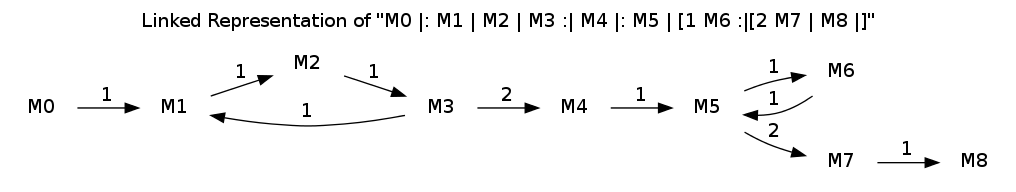
\includegraphics[width=\linewidth]{measure_example.png}

\section{ The Note class }
A Note contains a pitch and a duration  ( represented by a Fraction ).  It does NOT contain any information that refers to a larger data structure. The key signature / implicit accidentals, for instance, are not relevant. They should be handled by the Parser.

Rests are not notes, and in fact are not represented at all; they are redundant because note start times are explicitly specified by the Parser.

Notes are immutable objects.  Its values are pitch, length, accidentals, octave, and it has getter methods to access these values.  

\section{ Lexer }
The Lexer class will separate the input into tokens.  For the header of the piece, it will create field header tokens, field value tokens, and newline tokens to show the separation between fields and the header and body.  
For the body of the piece, it will create tokens for note pitches, which includes an upper or lowercase letter, accidental, or octave ticks, note length values, chords, tuples, rests, bar lines, and the symbols indicating that there are multiple voices.  It will also ignore whitespace.
The lexer will throw exceptions when it encounters invalid symbols or malformed tokens.  

\section{ Parser }


\section{ Visitor }

\section{ Testing }

\end{document}
